\subsection{Gráfico}

\begin{example}
    Considere as funções logarítmicas tais que $f(x) = \log_2 x$ e $g(x) = \log_{\frac 1 2} x$. Os gráficos de $f$ e $g$ são apresentados abaixo.
    \begin{figure}[H]
        \centering
        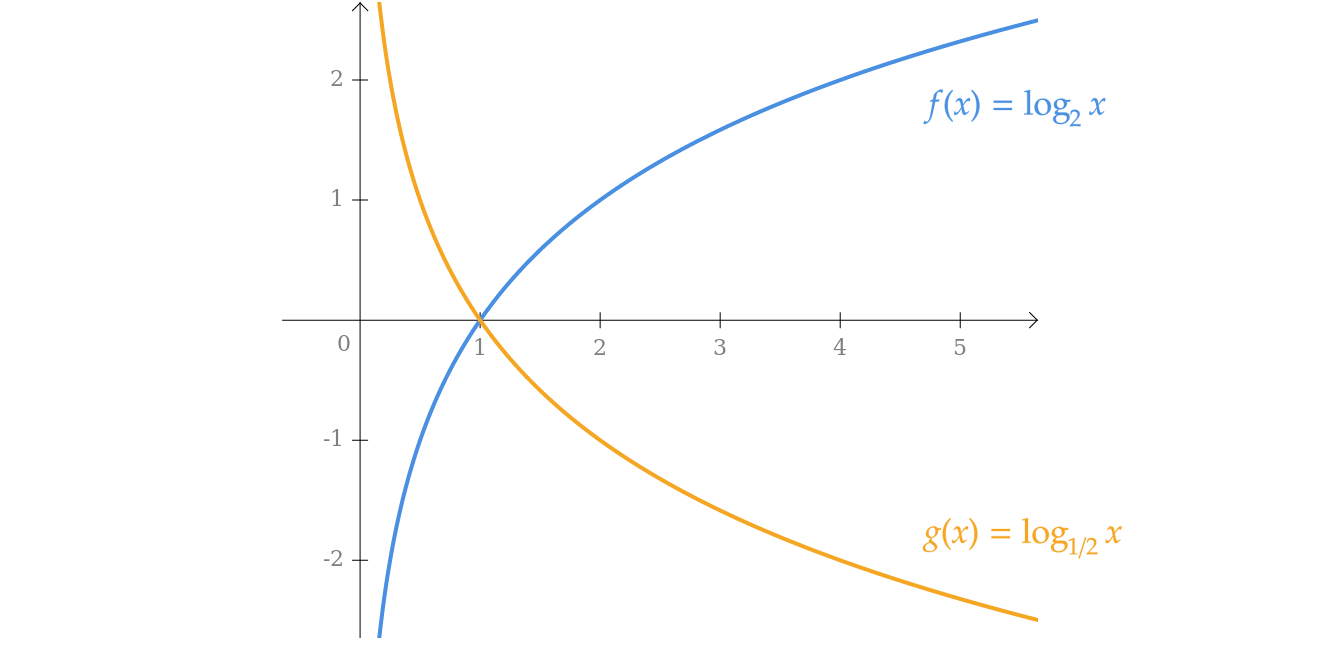
\includegraphics[scale=0.30]{\imgdirfromsection/grafico-logaritmica.png}
        \caption{Gráficos das funções $f$ e $g$.}
        \label{img:grafico-logaritmica}
    \end{figure}
\end{example}

Qual a relação entre os gráficos dessas funções?

\begin{solution}
    De modo geral, o gráfico de $h(x) = \log_b x$ terá forma semelhante ao de $f$ quando $b>1$, e semelhante
    ao de  $g$ quando $0<b<1$. Agora, verificaremos que o gráfico de $g$ é um reflexo vertical do gráfico de $f$,
    ou seja, $g(x) =  -f(x)$, para todo $x \in \preais$. Seja $x \in \preais$.
    Note que:
    %
    $$g(x) = \log_{\frac 1 2} x = \frac{\log_2 x}{\log_{\frac 1 2} 2}= \frac{\log_2 x}{\log_2 2^{-1}}=\frac{\log_2 x}{-1}=-f(x) $$
    %
    Assim, o gráfico de $g(x)$ é, simplesmente, uma reflexão do gráfico de $f(x)$. Mais geralmente,
    se $f$ e $g$ são funções logarítmicas de base $a$ e $b$, respectivamente, então $a\cdot b = 1$ se,
    e somente se, o gráfico de $g$ é reflexo vertical do gráfico de $f$ (exercício para o leitor).
\end{solution}

\begin{remark}
    Já vimos que o crescimento exponencial supera o de qualquer polinômio. Por ser a inversa da função exponencial, a função logarítmica possui um crescimento muito lento. Mesmo assim, a função logarítmica é ilimitada superiormente. Compare os gráficos abaixo:
\end{remark}

\begin{figure}[H]
    \centering
    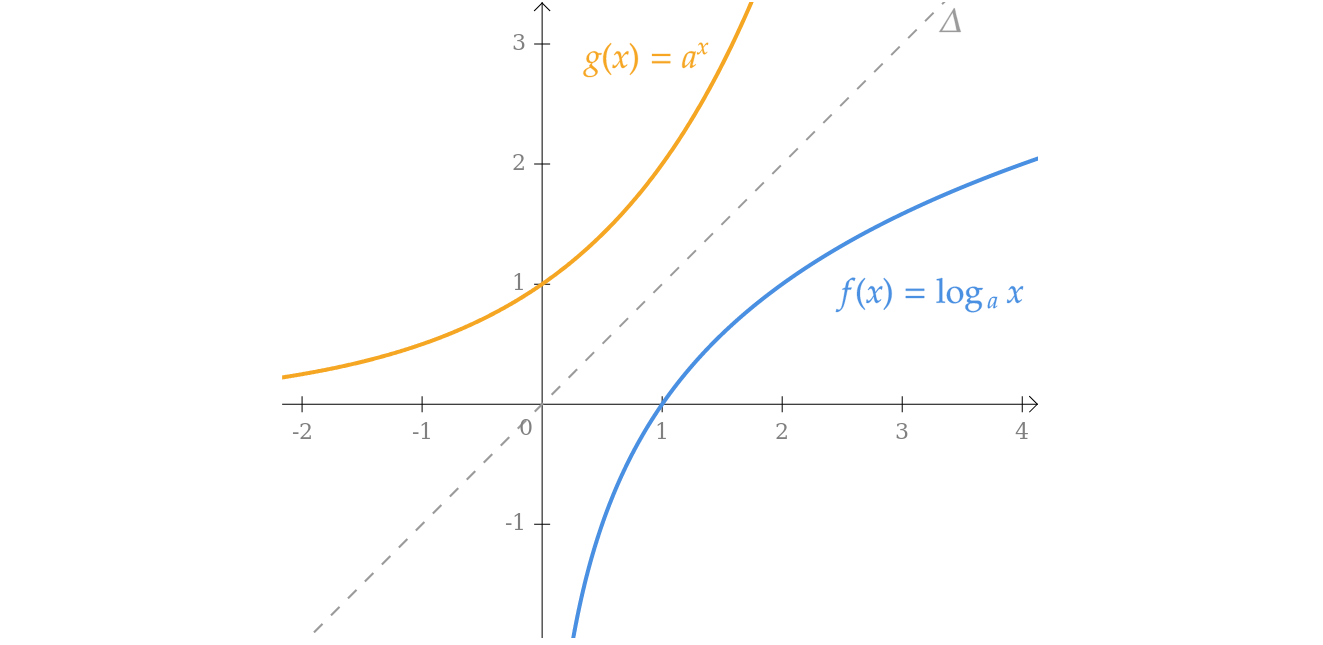
\includegraphics[scale=0.30]{\imgdirfromsection/logaritmica-vs-exponencial.png}
    \caption{Gráficos das funções $f$ e $g$.}
    \label{img:logaritmica-vs-exponencial}
\end{figure}

\begin{onlineact}
    \khan{https://pt.khanacademy.org/math/algebra2/exponential-and-logarithmic-functions/graphs-of-logarithmic-functions/e/graphs-of-exponentials-and-logarithms}{Gráficos de Funções Logarítmicas}
\end{onlineact}